\documentclass[nojss]{jss}\usepackage[]{graphicx}\usepackage[]{color}
%% maxwidth is the original width if it is less than linewidth
%% otherwise use linewidth (to make sure the graphics do not exceed the margin)
\makeatletter
\def\maxwidth{ %
  \ifdim\Gin@nat@width>\linewidth
    \linewidth
  \else
    \Gin@nat@width
  \fi
}
\makeatother

\definecolor{fgcolor}{rgb}{0.345, 0.345, 0.345}
\newcommand{\hlnum}[1]{\textcolor[rgb]{0.686,0.059,0.569}{#1}}%
\newcommand{\hlstr}[1]{\textcolor[rgb]{0.192,0.494,0.8}{#1}}%
\newcommand{\hlcom}[1]{\textcolor[rgb]{0.678,0.584,0.686}{\textit{#1}}}%
\newcommand{\hlopt}[1]{\textcolor[rgb]{0,0,0}{#1}}%
\newcommand{\hlstd}[1]{\textcolor[rgb]{0.345,0.345,0.345}{#1}}%
\newcommand{\hlkwa}[1]{\textcolor[rgb]{0.161,0.373,0.58}{\textbf{#1}}}%
\newcommand{\hlkwb}[1]{\textcolor[rgb]{0.69,0.353,0.396}{#1}}%
\newcommand{\hlkwc}[1]{\textcolor[rgb]{0.333,0.667,0.333}{#1}}%
\newcommand{\hlkwd}[1]{\textcolor[rgb]{0.737,0.353,0.396}{\textbf{#1}}}%

\usepackage{framed}
\makeatletter
\newenvironment{kframe}{%
 \def\at@end@of@kframe{}%
 \ifinner\ifhmode%
  \def\at@end@of@kframe{\end{minipage}}%
  \begin{minipage}{\columnwidth}%
 \fi\fi%
 \def\FrameCommand##1{\hskip\@totalleftmargin \hskip-\fboxsep
 \colorbox{shadecolor}{##1}\hskip-\fboxsep
     % There is no \\@totalrightmargin, so:
     \hskip-\linewidth \hskip-\@totalleftmargin \hskip\columnwidth}%
 \MakeFramed {\advance\hsize-\width
   \@totalleftmargin\z@ \linewidth\hsize
   \@setminipage}}%
 {\par\unskip\endMakeFramed%
 \at@end@of@kframe}
\makeatother

\definecolor{shadecolor}{rgb}{.97, .97, .97}
\definecolor{messagecolor}{rgb}{0, 0, 0}
\definecolor{warningcolor}{rgb}{1, 0, 1}
\definecolor{errorcolor}{rgb}{1, 0, 0}
\newenvironment{knitrout}{}{} % an empty environment to be redefined in TeX

\usepackage{alltt}

%%%%%%%%%%%%%%%%%%%%%%%%%%%%%%
%% declarations for jss.cls %%
%%%%%%%%%%%%%%%%%%%%%%%%%%%%%%
%\VignetteEngine{knitr::knitr}
%\VignetteIndexEntry{hviPlotR}
%\VignetteIndexEntry{hviPlotR: Generating plot.sas style figures in R}
%\VignetteKeywords{publication, manuscript, powerpoint, ggplot2, plot.sas}
%\VignetteDepends{hviPlotR}
%\VignettePackage{hviPlotR} 

\usepackage{float}
\usepackage{listings}
\usepackage{color}

\definecolor{mygreen}{rgb}{0,0.6,0}
\definecolor{mygray}{rgb}{0.95,0.95,0.95}
\definecolor{mymauve}{rgb}{0.58,0,0.82}
\lstset{
backgroundcolor=\color{white},   % choose the background color; you must add \usepackage{color} or \usepackage{xcolor}
basicstyle=\ttfamily\footnotesize,
breakatwhitespace=false,         % sets if automatic breaks should only happen at whitespace
breaklines=true,                 % sets automatic line breaking
captionpos=b,                    % sets the caption-position to bottom
commentstyle=\color{mygreen},    % comment style
%deletekeywords={...},            % if you want to delete keywords from the given language
escapeinside={\%*}{*)},          % if you want to add LaTeX within your code
extendedchars=true,              % lets you use non-ASCII characters; for 8-bits encodings only, does not work with UTF-8
%frame=single,                    % adds a frame around the code
keepspaces=true,                 % keeps spaces in text, useful for keeping indentation of code (possibly needs columns=flexible)
keywordstyle=\color{blue},       % keyword style
language={SAS},                  % the language of the code
morekeywords={*,...},            % if you want to add more keywords to the set
numbers=none,                    % where to put the line-numbers; possible values are (none, left, right)
%numbersep=5pt,                   % how far the line-numbers are from the code
%numberstyle=\tiny\color{mygray}, % the style that is used for the line-numbers
%rulecolor=\color{black},         % if not set, the frame-color may be changed on line-breaks within not-black text (e.g. comments (green here))
showspaces=false,                % show spaces everywhere adding particular underscores; it overrides 'showstringspaces'
showstringspaces=false,          % underline spaces within strings only
showtabs=false,                  % show tabs within strings adding particular underscores
%stepnumber=2,                    % the step between two line-numbers. If it's 1, each line will be numbered
stringstyle=\color{mymauve},     % string literal style
tabsize=2,                       % sets default tabsize to 2 spaces
title=\lstname                   % show the filename of files included with \lstinputlisting; also try caption instead of title
}

%% almost as usual
\author{John Ehrlinger\\Quantitative Health Sciences\\Lerner Research Institute\\Cleveland Clinic} %\And \\Plus Affiliation}
\title{The {\pkg{hviPlotR}} package: Generating \code{plot.sas} style figures in \proglang{R}}

%% for pretty printing and a nice hypersummary also set:
\Plainauthor{John Ehrlinger} %% comma-separated
\Plaintitle{hviPlotR: Generating plot.sas style figures in R} %% without formatting
\Shorttitle{hviPlotR: Generating plot.sas style figures}
\Submitdate{\today}
%% an abstract and keywords
\Abstract{ 
We introduce the \proglang{R} package \pkg{hviPlotR}, tools for creating publication quality graphics in \proglang{R} for the Heart \& Vascular Institute Clinical Investigations statistics group at the Cleveland Clinic. The \pkg{hviPlotR} package contains a tutorial for generating figures (this vignette) and small set of functions for formatting and saving those figures. These tools describe how to generate figures in \proglang{R} to replace the \code{plot.sas} macro we currently use in \proglang{SAS}.

This package vignette is a tutorial for generating our standard figures using the \pkg{ggplot2} package commands in \proglang{R}. The tutorial presents a series of \proglang{R} recipes for generating figures. The \pkg{hviPlotR} package includes a set of themes designed to format those figures for inclusion in manuscript and \code{PowerPoint} targets. 

This document is included with the \pkg{hviPlotR} package as a package vignette. The vignette is installed into \proglang{R} when the \pkg{hviPlotR} package is installed, and viewable using the \code{vignette("hviPlotR")} command. The goal of the vignette is as a tutorial to document the best practices of creating our publication quality graphics for both manuscripts and power point presentations. It is our intent to update this vignette as our standards and the \pkg{hviPlotR} package are modified.
}
\Keywords{publication graphics, powerpoint, ggplot2, plot.sas}
\Plainkeywords{publication graphics, powerpoint, ggplot2, plot.sas}
%% at least one keyword must be supplied

%% publication information
%% NOTE: Typically, this can be left commented and will be filled out by the technical editor
%% \Volume{13}
%% \Issue{9}
%% \Month{September}
%% \Year{2004}
%% \Submitdate{2004-09-29}
%% \Acceptdate{2004-09-29}

%% The address of (at least) one author should be given
%% in the following format:
\Address{
John Ehrlinger\\
Quantitative Health Sciences\\
Lerner Research Institute\\
Cleveland Clinic\\
9500 Euclid Ave\\
Cleveland, Ohio 44195\\
%  Telephone: +41/0/44634-4643 \\
%  Fax: +41/0/44634-4386 \\
E-mail: \email{john.ehrlinger@gmail.com}\\
URL: \url{http://www.lerner.ccf.org/qhs/people/ehrlinj/}\\
URL: \url{https://github.com/ehrlinger/hviPlotR}
}

%% It is also possible to add a telephone and fax number
%% before the e-mail in the following format:
%% Telephone: +43/1/31336-5053
%% Fax: +43/1/31336-734

%% for those who use Sweave please include the following line (with % symbols):
%% need no \usepackage{Sweave.sty}

%% end of declarations %%%%%%%%%%%%%%%%%%%%%%%%%%%%%%%%%%%%%%%%%%%%%%%



\IfFileExists{upquote.sty}{\usepackage{upquote}}{}
\begin{document}

%% include your article here, just as usual
%% Note that you should use the \pkg{}, \proglang{} and \code{} commands.

\begin{knitrout}\footnotesize
\definecolor{shadecolor}{rgb}{0.969, 0.969, 0.969}\color{fgcolor}\begin{figure}[htpb]

{\centering 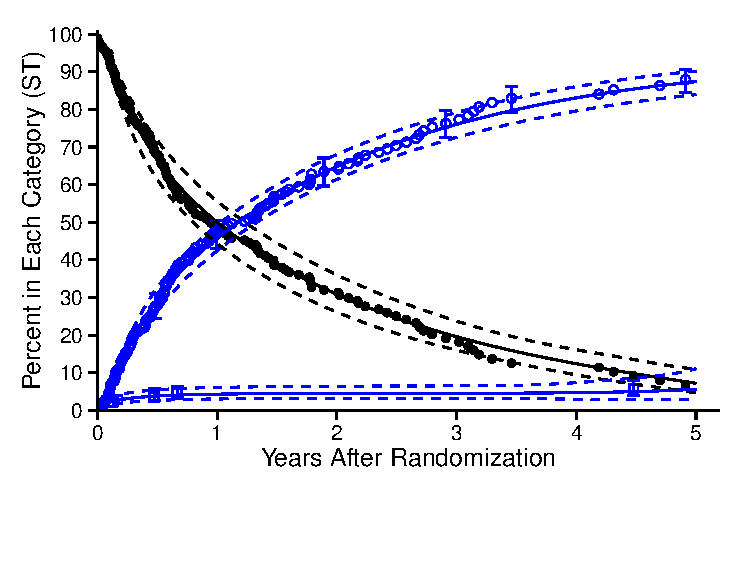
\includegraphics[width=\maxwidth]{figure/beamer-introFigure-1} 

}

\caption[Demonstration figure]{Demonstration figure\label{F:introFigure}}
\end{figure}


\end{knitrout}

% -----------------------------------------------------
\section*{About this document}
% -----------------------------------------------------
This package vignette is an introduction to the \proglang{R} package \pkg{hviPlotR}, and a tutorial for creating publication quality graphics in \proglang{R}. The package and this document describe the process of creating graphics in \proglang{R} that conform to the standards of the clinical investigations statistics group within The Heart \& Vascular Institute at the Cleveland Clinic. These graphics are analogous to those generated with the \code{plot.sas} macro in \proglang{SAS}.

The document is a package vignette for the \pkg{hviPlotR} package, and is the primary documentation for the package. The latest version of the document can be obtained with the following command: 
\begin{CodeChunk}
\begin{CodeInput}
R> vignette("hviPlotR", package = "hviPlotR")
\end{CodeInput}
\end{CodeChunk}

The goal is to update this vignette as the package, and our graphing standards, are updated. A development version of the \pkg{hviPlotR} package is also available on Github (\url{https://github.com}). We invite comments, feature requests and bug reports for this package at \url{https://github.com/ehrlinger/hviPlotR}.

% -----------------------------------------------------
\section{Introduction}
% -----------------------------------------------------
For many years, the mainstay for generating graphics for manuscripts and presentations in the statistics group in The Heart \& Vascular Institute has been the \code{plot.sas} macro using \proglang{SAS}. However, recently, we have had issues migrating this macro to newer versions of \proglang{SAS} ($> 8.0$) and Microsoft Office products ($> 2003$). 

In an effort to alleviate these version issues, and to standardize the generation of figures within \proglang{R}, we have developed the \pkg{hviPlotR} \proglang{R} package. The goal of the package, and this vignette, is simplify the creation of publication quality graphics in  \proglang{R}. We are specifically encoding the best practices of the HVI Clinical Investigations formatting, so that our statisticians will be able to create graphics for publications and presentations with a minimal amount of effort.

The \pkg{hviPlotR} package implements best practices for \proglang{R} graphics by leveraging the \pkg{ggplot2} package~\citep{Wickham:2009}. The \pkg{ggplot2} package is an implementation of the Grammar of Graphics~\citep{Wilkinson:2005}, which is a formalization of graphical concepts, and the building of graphical objects from a sequence of independent components. These components can be combined in many different ways.

The \code{plot.sas} macro is also an implementation of a graphics grammar. The grammar \code{plot.sas} is derived from the ZETA pen plotters, which used GML (Graphics Machine Language) to control between 4 and and 8 colored pens for generating color line and point figures. Because both systems use a graphics language it is a straight forward exercise to translate commands between the two systems. 

This document outlines how to generate figures using the \pkg{ggplot2} package in \proglang{R}. Our approach is to demonstrate the \proglang{R} commands to generate the same elements created with \code{plot.sas} commands. Section~\ref{S:plot.sas} gives an overview of the methodology of the \code{plot.sas} macro and Section~\ref{S:ggplot2tuple} details how to create line and point plots with similar \pkg{ggplot2} commands. 

The \pkg{hviPlotR} package contains custom themes for figures. Once a figure has been created using \pkg{ggplot2} commands, Section~\ref{S:themes} details how to use the themes contained in the \pkg{hviPlotR} package to get the formatting correct for manuscripts or presentations. Section~\ref{S:saving} describes how to save these figures to simplify the import into publication documents.


% -----------------------------------------------------
\section[The plot.sas macro]{The \code{plot.sas} macro}\label{S:plot.sas}
% -----------------------------------------------------

We first look at some example code using the \code{plot.sas} macro. This code is intended to generate a figure for manuscript publication and was modified to generate Figure~\ref{F:introFigure}. We will walk through this example code in this section to help us understand the steps for generating these figures in \proglang{R}.

\begin{lstlisting}[float,floatplacement=!htpb, caption={plot.sas commands: Figure setup.},label={plot.sas:figureSetup}]
%let STUDY=/studies/cardiac/valves/aortic/replacement/partner_publication_office/partner1b/mortality_5y
*****************************************************************************;
* Bring in PostScript plot macro                                             ;
filename plt "!MACROS/plot.sas"; %inc plt;
filename gsasfile pipe 'lp';
*____________________________________________________________________________;
*                                                                            ;
*                       P O S T S C R I P T   P L O T S
*____________________________________________________________________________;
* Multiple decrement, nonparametric and parametric                           ;
filename gsasfile "&STUDY/graphs/ce.states.ST.ps";

*____________________________________________________________________________;
* Create the figure here   !                                                 ;
*____________________________________________________________________________;
%plot(goptions gsfmode=replace, device=pscolor, gaccess=gsasfile end;
      id l="&STUDY/graphs/ce.states.ST.sas percent", end;
      labelx l="Years After Randomization", end;
      axisx order=(0 to 5 by 1), minor=none, end;
      labely l="Percent in Each Category (ST)", end;
      axisy order=(0 to 100 by 10), minor=none, end;
\end{lstlisting}

Note the first line of the code block in Listing~\ref{plot.sas:figureSetup} indicates the path to the specific example file location. The \code{filename} statements bring in the \code{plot.sas} macro, indicate how to print, and where to save the graphics file. The \code{plot.sas} macro call starts with the \code{\%plot} command. The \code{goptions} statement in the first line sets global graphic values, including the filename (\code{gaccess=}) where the figure will be saved (see Section~\ref{S:saving}). Each \code{plot.sas} command is terminated with the \code{end;} statement. We'll look at each of the remaining command type individually.

The \code{id l=} command sets the footnote text used for manuscript figures to identify where the figure is saved (see Section~\ref{S:saving}). The \code{labelx} and \code{labely} commands set the axis label text (Section~\ref{S:labels}) and the \code{axisx} and \code{axisy} set the scales for each axis locating text and tics (Section~\ref{S:scales}).

\begin{lstlisting}[float,floatplacement=!htpb, caption={plot.sas commands: points and errorbar tuple statements.}, label={plot.sas:pointTuple}]
     /******NON-PARAMETRIC: SYMBOLS AND CONFIDENCE BARS *******/
     tuple set=green, symbol=dot, symbsize=1/2, linepe=0, linecl=0,
          ebarsize=3/4, ebar=1,
          x=iv_state, y=sginit, cll=stlinit, clu=stuinit, color=black, 
          end;

     tuple set=green, symbol=circle, symbsize=1/2, linepe=0, linecl=0,
          ebarsize=3/4, ebar=1,
          x=iv_state, y=sgdead1, cll=stldead1, clu=studead1, color=blue, 
          end;
          
     tuple set=green, symbol=square, symbsize=1/2, linepe=0, linecl=0,
          ebarsize=3/4, ebar=1,
          x=iv_state, y=sgstrk1, cll=stlstrk1, clu=stustrk1, color=blue, 
          end;
\end{lstlisting}
The \code{plot.sas} continues in Listing~\ref{plot.sas:pointTuple}. Here, the \code{tuple} command builds up graphics objects within the figure plot window. This first set of \code{tuple} commands constructs a set of three elements containing both points (Section~\ref{S:points}) and errorbars (Section~\ref{S:errorbars}). Each \code{tuple} statement operates on the dataset indicated by the \code{set} command. Symbols shapes and sizes are specified with the \code{symbol} and \code{symbsize} commands (Section~\ref{S:shapes}).

The second set of \code{tuple} statements in Listing~\ref{plot.sas:linesTuple} construct a set of three elements containing lines and confidence intervals (Section~\ref{S:lines}).
\begin{lstlisting}[float,floatplacement=!htpb, caption={plot.sas commands: lines tuple statements.}, label={plot.sas:linesTuple}]
     /**********PARAMETRIC : SOLID LINES AND CONFIDENCE INTERVALS**********/      
     tuple set=all, x=years, y=noinit, cll=clinit, clu=cuinit,
          width=0.5,color=black, 
          end;
     
     tuple set=all, x=years, y=nodeath, cll=cldeath, clu=cudeath,
          width=0.5,color=blue, 
          end;

     tuple set=all, x=years, y=nostrk, cll=clstrk, clu=custrk,
          linecl=2, width=0.5,color=blue, 
          end;
);
run;
\end{lstlisting}

The \code{plot.sas} macro code is closed by the ending \code{);} characters, and \proglang{SAS} is instructed to \code{run;} the code. Running combines building the figure by combining elements from \code{label}, \code{axis} and \code{tuple} statements and saving it into the file specified by the \code{gsasfile} variable. The resulting figure is shown in Figure~\ref{F:sasManuscript}.

\begin{figure}[!htpb]
\centering
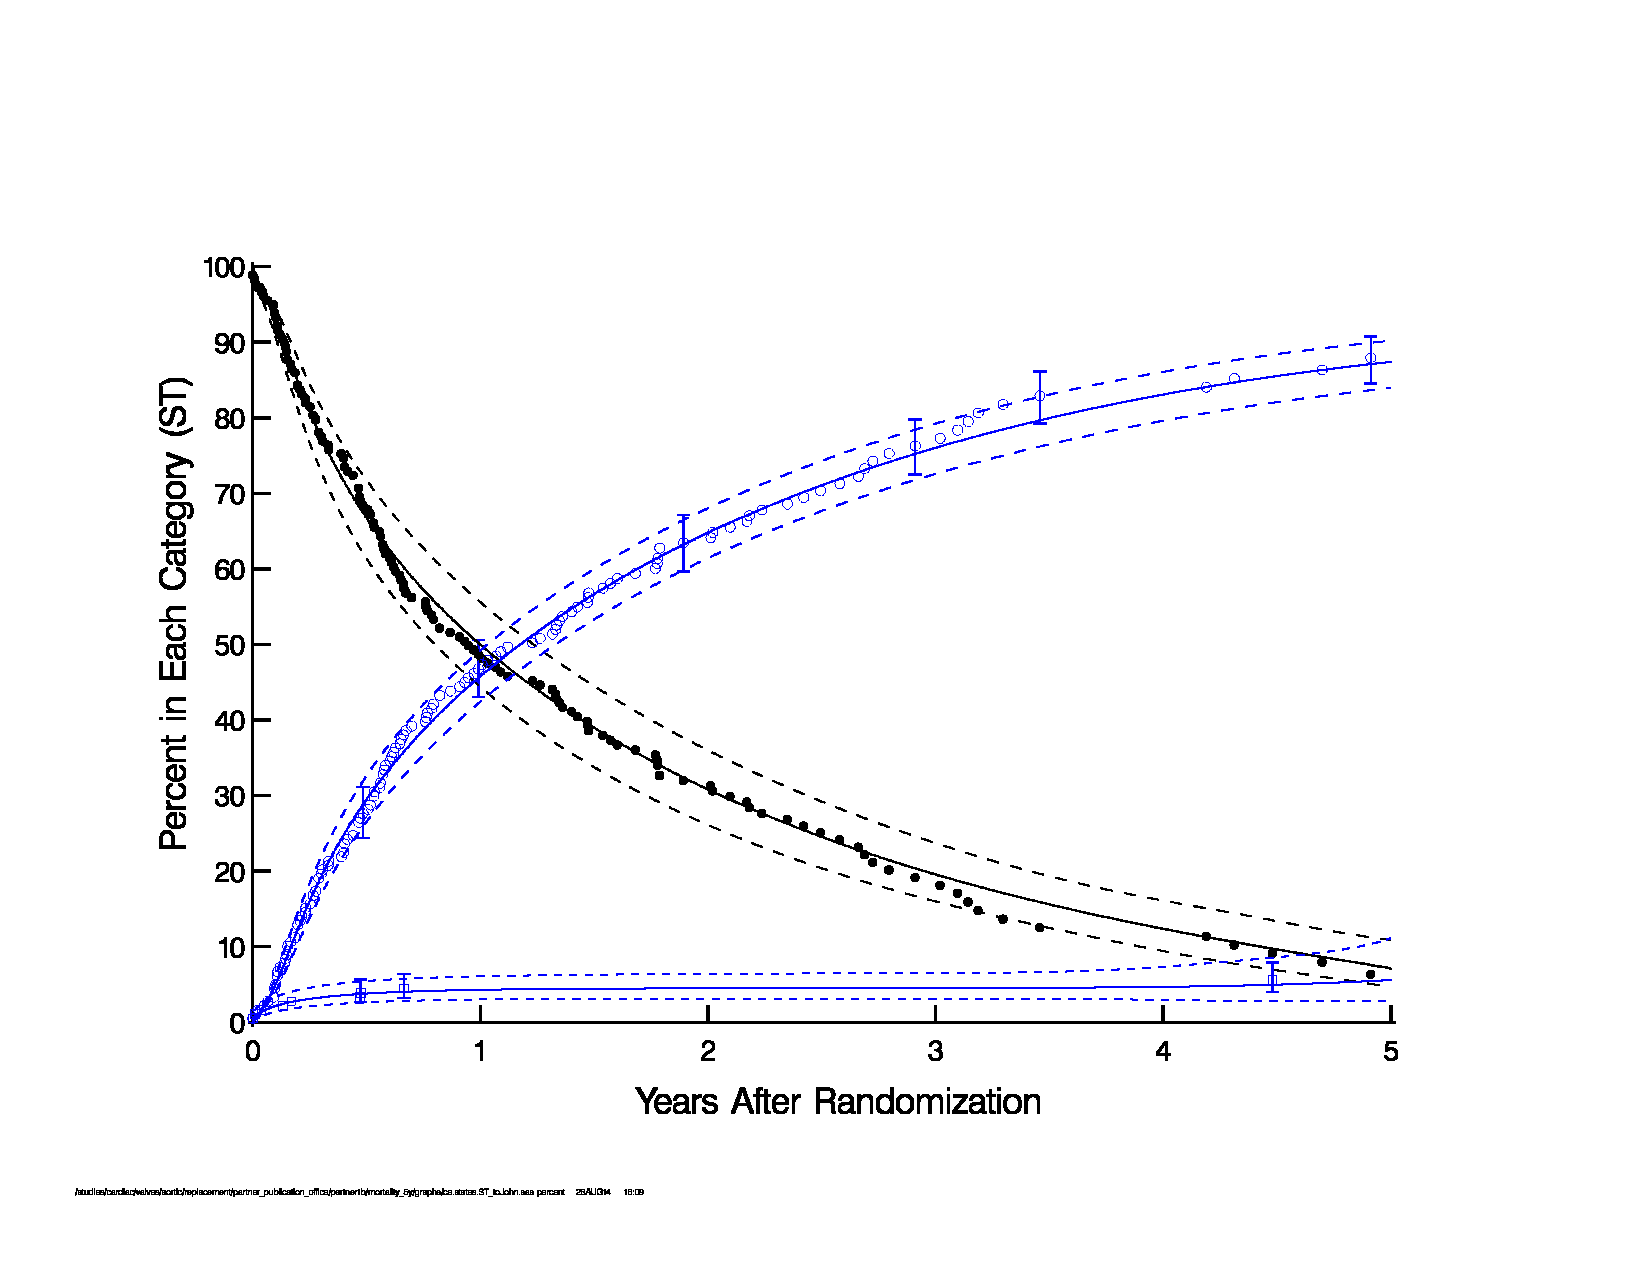
\includegraphics[width=0.8\textwidth]{../inst/ceStatesST.pdf}
\caption{Manuscript figure (SAS version)}
\label{F:sasManuscript}
\end{figure}

Note that much of the figure formatting is mixed within the \code{tuple} statements using \code{width}, \code{color}, \code{linepe} and \code{linecl} commands. In the \code{plot.sas} macro, omitting these commands will generate a figure with the default values specified within the \code{plot.sas} macro or \code{device} theme (Section~\ref{S:themes}).

\begin{lstlisting}[float,floatplacement=!htpb, caption={plot.sas commands: PowerPoint graphics using CGM instructions.}, label={plot.sas:cgm}]
*____________________________________________________________________________;
*                                                                            ;
*       C G M   F I L E S   F O R   P O W E R P O I N T   S L I D E S
*____________________________________________________________________________;
* Competing risks, parametric only                                           ;
filename gsasfile "&STUDY/graphs/ce.states.ST.cgm";
%plot(goptions gsfmode=replace, device=cgmmppa, ftext=hwcgm001, end;
     axisx order=(0 to 5 by 1), minor=none, value=(height=2.4), end;
     axisy order=(0 to 100 by 20), minor=none, value=(height=2.4), 
     value=(height=2.4 j=r ' ' '20' '40' '60' '80' '100'), end;
     tuple set=all, x=years, y=noinit, width=3, color=gray, end;
     tuple set=all, x=years, y=nostrk, width=3, color=red, end;
     tuple set=all, x=years, y=nodeath, width=3, color=blue, end;
);
run;  
\end{lstlisting}

A similar set of \code{plot.sas} commands (Listing~\ref{plot.sas:cgm}) is used to create presentation graphics.
Differences between manuscript and presentation graphics include the target \code{device} and \code{ftext} as well as some handling of figure labels with \code{value} instead of \code{label} commands. The output from this code is shown in Figure~\ref{F:sasPowerPoint}. 

\begin{figure}[!htpb]
\centering
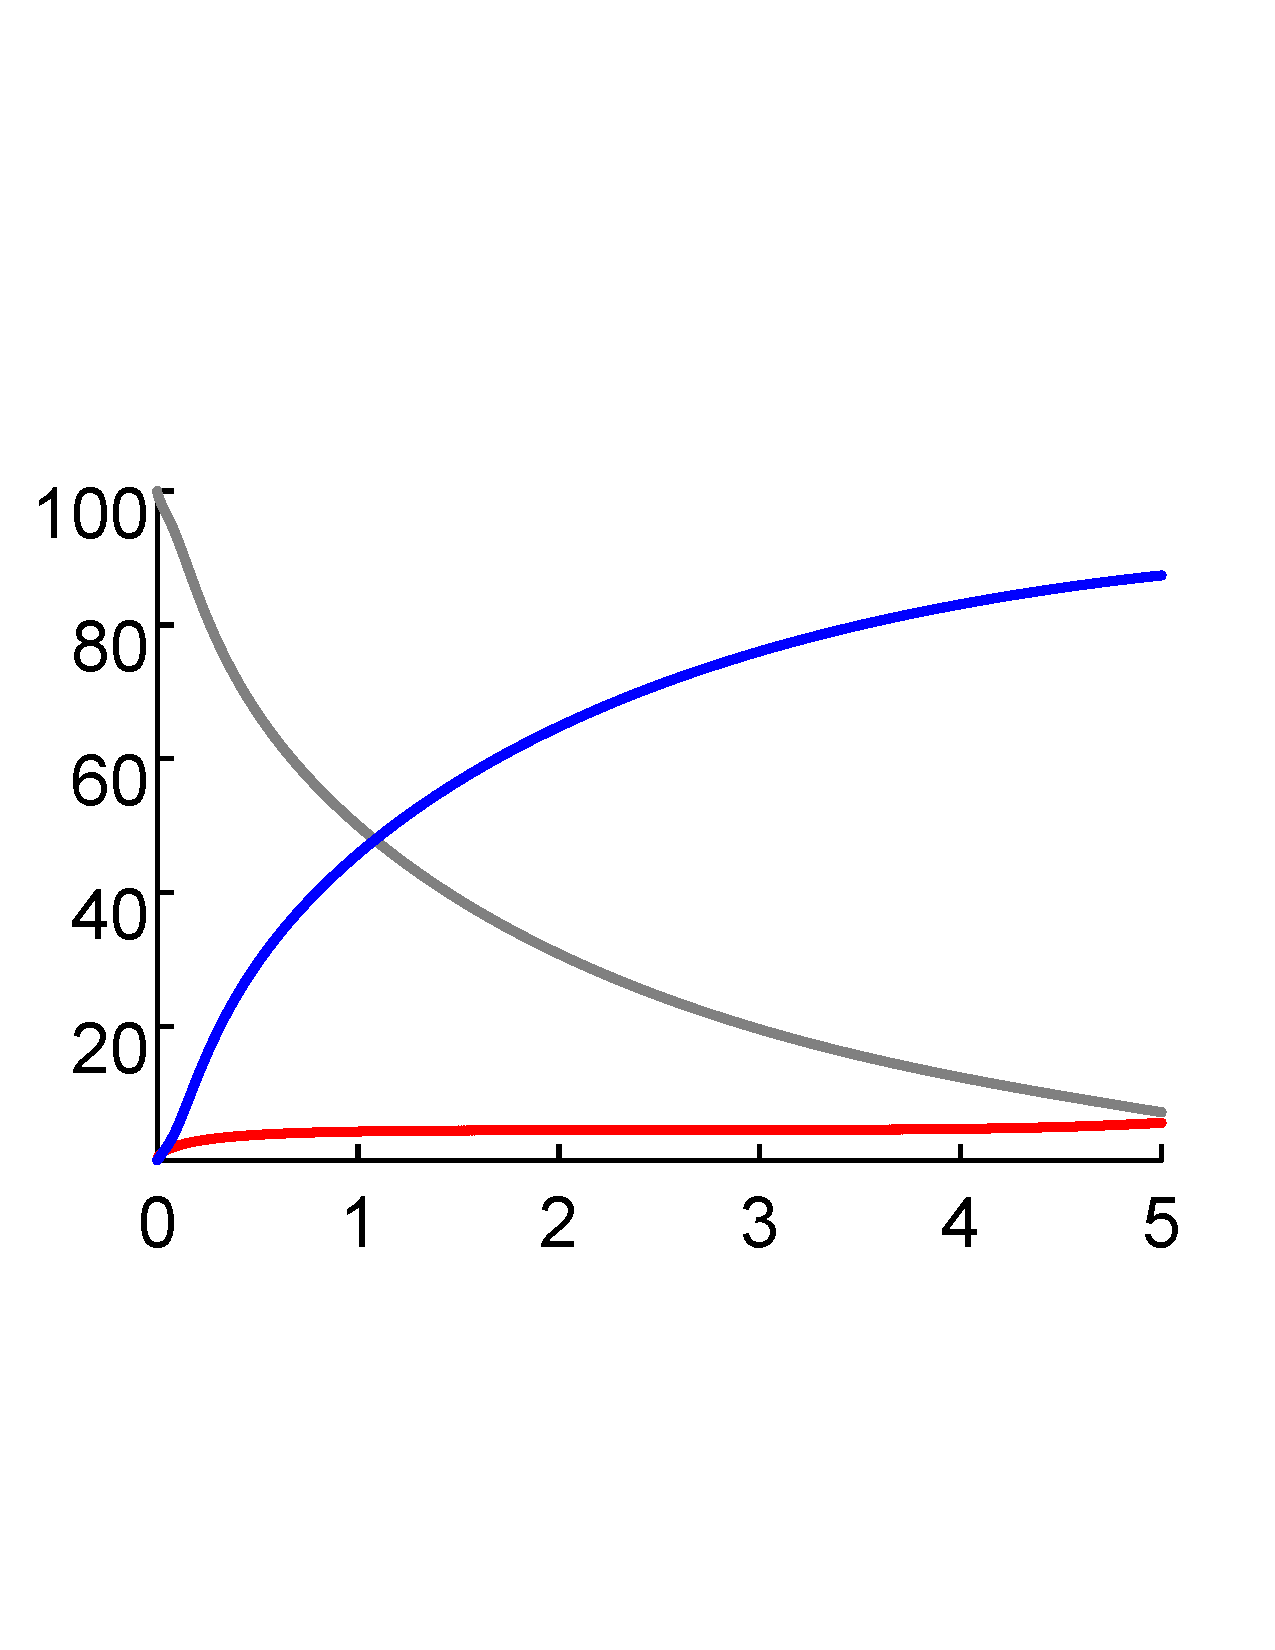
\includegraphics[width=0.8\textwidth]{../inst/ceStatesST_ppt.pdf}
\caption{PowerPoint figure (SAS version)}
\label{F:sasPowerPoint}
\end{figure}

In addition to the \code{plot.sas} commands, we also have a set of graphics standards (graphics rules) for what to and not to include in presentation graphics, we will describe these rules in (Section~\ref{S:rules}). Many of these are incorporated into the \code{plot.sas} macro to protect the user from violating these standards.

% -----------------------------------------------------
\section[Generating ggplot2 graphics]{Generating \pkg{ggplot2} graphics}\label{S:ggplot2tuple}
% -----------------------------------------------------

In order to create figures similar to using \code{plot.sas} macro, using \proglang{R}, we will make extensive use of the \pkg{ggplot2} package. This will require translating from the graphics language of \code{plot.sas} to the graphics language of \pkg{ggplot2}. 

For the remainder of this document, \proglang{R} code will be highlighted in grey boxes, as shown below. We will refer to these blocks as \emph{code chunks}. You can run each code chunk individually, using copy/paste into an interactive \proglang{R} session, or within a stand alone \proglang{R} script.

This tutorial requires the \pkg{hviPlotR} package to load the data and themes we will be discussing. You can install the package with the following commands:
\begin{knitrout}\footnotesize
\definecolor{shadecolor}{rgb}{0.969, 0.969, 0.969}\color{fgcolor}\begin{kframe}
\begin{alltt}
\hlcom{# Install the latest hviPlotR package.}
\hlcom{#}
\hlcom{# The devtools package is installed on all our }
\hlcom{# jjnb-gen servers as well as other R instances.}
\hlcom{#}
\hlcom{# For working on your own install, first use the install command}
\hlcom{# install.packages("devtools")}

\hlcom{# Load the package}
\hlkwd{library}\hlstd{(devtools)}

\hlcom{# To get the latest version of hviPlotR.}
\hlkwd{install_github}\hlstd{(}\hlstr{"ehrlinger/hviPlotR"}\hlstd{)}
\end{alltt}
\end{kframe}
\end{knitrout}

\subsection{Importing the data}\label{S:sasData}
For most of this document, we assume that the data analysis has been completed in \proglang{SAS}. In this case, the first step in creating figures in \proglang{R} is to get the data out of \proglang{SAS}. There are many ways to do this, but we have had success using the \code{tp.bd.SAStoR.sas} program (under the \code{datasets} folder) to export a data set into a \proglang{SAS} \code{xport} file.

Once an \code{xport} file has been created, we read it into \proglang{R} with the \pkg{foreign} package. This recipe reads an \code{xport} into a \code{data.frame} and then re-reads the \code{xport} file to pull out the \proglang{SAS} labels to describe the variables. The labels will be stored in a vector, which we can index by the variable names.


\begin{knitrout}\footnotesize
\definecolor{shadecolor}{rgb}{0.969, 0.969, 0.969}\color{fgcolor}\begin{kframe}
\begin{alltt}
\hlkwd{library}\hlstd{(foreign)}

\hlcom{# The xport file name}
\hlstd{dtFilename} \hlkwb{=} \hlstr{"../datasets/par_cst.xpt"}

\hlcom{# Read the xport file into a data.frame}
\hlstd{dta}\hlkwb{<-} \hlkwd{read.xport}\hlstd{(dtFilename)}

\hlcom{# Reading in the labels takes 2 more commands.}
\hlstd{dta.info} \hlkwb{<-} \hlkwd{lookup.xport}\hlstd{(dtFilename)}
\hlstd{dta.labels} \hlkwb{<-} \hlstd{dta.info[[}\hlnum{1}\hlstd{]]}\hlopt{$}\hlstd{label}

\hlcom{## Fill in empty labels with the variable name}
\hlstd{dta.labels}\hlkwb{<-}\hlkwd{sapply}\hlstd{(}\hlnum{1}\hlopt{:}\hlkwd{length}\hlstd{(dta.labels),} \hlkwa{function}\hlstd{(}\hlkwc{ind}\hlstd{)\{}
  \hlkwa{if}\hlstd{(dta.labels[ind]} \hlopt{==} \hlstr{""}\hlstd{)}
    \hlkwd{colnames}\hlstd{(dta)[ind]}
  \hlkwa{else}
    \hlstd{dta.labels[ind]}
\hlstd{\})}

\hlcom{## For indexing the labels, }
\hlkwd{names}\hlstd{(dta.labels)} \hlkwb{=} \hlkwd{colnames}\hlstd{(dta)}
\end{alltt}
\end{kframe}
\end{knitrout}

\subsection{Initialize the figure}\label{S:initial}
Referring back to the \proglang{SAS} code chunks in Section~\ref{S:plot.sas},  Listing~\ref{plot.sas:figureSetup} sets the current working directory, and does some house keeping, including loading the \code{plot.sas} macro. Similarly, to get started in \proglang{R}, we first load the required libraries: \pkg{ggplot2} for graphics, and \pkg{hviPlotR} for themes. The following code chunk also sets the initial default theme to a generic black and white format, and brings in a pair of example datasets. 
\begin{knitrout}\footnotesize
\definecolor{shadecolor}{rgb}{0.969, 0.969, 0.969}\color{fgcolor}\begin{kframe}
\begin{alltt}
\hlcom{# load required libraries}
\hlkwd{library}\hlstd{(ggplot2)}   \hlcom{# Plotting environment}
\hlkwd{library}\hlstd{(hviPlotR)}  \hlcom{# CCF HVI plotting functionality }

\hlkwd{theme_set}\hlstd{(}\hlkwd{theme_bw}\hlstd{())} \hlcom{# A reasonable default plotting theme}

\hlcom{# Load the example datasets }
\hlkwd{data}\hlstd{(parametric,} \hlkwc{package}\hlstd{=}\hlstr{"hviPlotR"}\hlstd{)}
\hlkwd{data}\hlstd{(nonparametric,} \hlkwc{package}\hlstd{=}\hlstr{"hviPlotR"}\hlstd{)}
\end{alltt}
\end{kframe}
\end{knitrout}

One advantage of \pkg{ggplot2} is that figures can be built up in successive statements. This tutorial will make extensive use of this to demonstrate the process. Starting in this code chunk, we will save the intermediate objects in the \code{ccf_plot} variable. Here we simply create an empty \pkg{ggplot2} figure that we will be adding to as we work through the commands in the \code{plot.sas} macro. Note that we include the \code{\%plot()} commands in the comments above the equivalent \pkg{ggplot2} command for comparison.
\begin{knitrout}\footnotesize
\definecolor{shadecolor}{rgb}{0.969, 0.969, 0.969}\color{fgcolor}\begin{kframe}
\begin{alltt}
\hlcom{## To reproduce the plot.sas function, line by line.}
\hlcom{###-------------}
\hlcom{## There are SAS options we will not use here.}
\hlcom{#}
\hlcom{#  %plot(goptions gsfmode=replace, device=pscolor, gaccess=gsasfile end;}
\hlstd{ccf_plot} \hlkwb{<-} \hlkwd{ggplot}\hlstd{()}
\end{alltt}
\end{kframe}
\end{knitrout}

In \proglang{R}, we set the equivalent variables \code{gsmode}, \code{device} and \code{gaccess} when saving the figure (Section~\ref{S:saving}).

\subsection{Labels}\label{S:labels}
The next section of Listing~\ref{plot.sas:figureSetup} in Section~\ref{S:plot.sas} sets the x and y axis titles, as well as the location of the major axis tick marks. We will split this up in our \proglang{R} code. The \pkg{ggplot2} package uses the \code{labs} function to set the axis labels. 
\begin{knitrout}\footnotesize
\definecolor{shadecolor}{rgb}{0.969, 0.969, 0.969}\color{fgcolor}\begin{kframe}
\begin{alltt}
\hlcom{###-------------}
\hlcom{## Labels are a single command, scales control the axis}
\hlcom{#}
\hlcom{#    labelx l="Years After Randomization", end;}
\hlcom{#    labely l="Percent in Each Category (ST)", end;}
\hlstd{ccf_plot} \hlkwb{<-} \hlstd{ccf_plot} \hlopt{+}
  \hlkwd{labs}\hlstd{(}\hlkwc{x}\hlstd{=}\hlstr{"Years After Randomization"}\hlstd{,}
       \hlkwc{y}\hlstd{=}\hlstr{"Percent in Each Category (ST)"}\hlstd{)}
\end{alltt}
\end{kframe}
\end{knitrout}

The \code{labs} function can also be used to set the plot \code{title} and legend titles. We will not cover that functionality here, details are available in~\cite{Wickham:2009} or through the Internet.

\subsection{Scales}\label{S:scales}
Axis ticks are controlled with the \code{scale_} functions. \pkg{ggplot2} has many different \code{scale_} functions. These functions will work on one axis at a time, so for a typical continuous axis, we use the \code{scale_x_continuous} or \code{scale_y_continuous} functions. Major axis are controlled using the \code{breaks} argument. Listing~\ref{plot.sas:figureSetup} uses a sequence of numbers to set the location of major tick marks (\code{seq(0,5,1)}). One mark for every year starting at 0, and ending at 5. Minor tick marks are automatically generated, but can also be specified using a \code{minor_breaks=} argument. You could also specify the breaks using a vector of values (\code{c(0,1,2,3,4,5)}), as well as relabel the ticks manually using a \code{labels=} argument.

Note that the \code{scale_} functions do not restrict the figure viewport at all. They are simply used to setup and label the axis tick marks. You can specify that the y-axis ticks are only from 0 to 50, and the figure would have a blank axis from 50 to the limits of the data. We discuss controlling the figure viewport in Section~\ref{S:globals}.

\begin{knitrout}\footnotesize
\definecolor{shadecolor}{rgb}{0.969, 0.969, 0.969}\color{fgcolor}\begin{kframe}
\begin{alltt}
\hlcom{###-------------}
\hlcom{## Labels are a single command, scales control the axis}
\hlcom{#}
\hlcom{#      axisx order=(0 to 5 by 1), minor=none, end;}
\hlcom{#      axisy order=(0 to 100 by 10), minor=none, end;}
\hlstd{ccf_plot} \hlkwb{<-} \hlstd{ccf_plot} \hlopt{+}
  \hlkwd{scale_x_continuous}\hlstd{(}\hlkwc{breaks}\hlstd{=}\hlkwd{seq}\hlstd{(}\hlnum{0}\hlstd{,}\hlnum{5}\hlstd{,}\hlnum{1}\hlstd{))}\hlopt{+}
  \hlkwd{scale_y_continuous}\hlstd{(}\hlkwc{breaks}\hlstd{=}\hlkwd{seq}\hlstd{(}\hlnum{0}\hlstd{,}\hlnum{100}\hlstd{,}\hlnum{10}\hlstd{))}
\end{alltt}
\end{kframe}
\end{knitrout}

Up to this point, we have only created and \emph{decorated} the plot object stored in the \code{ccf_plot} variable. Showing the figure (\code{show()}) or saving the figure would result in an error, since we have not added any data to the object, or described how we want it displayed. 

\subsection{Points}\label{S:points}

The fundamental statement of the \code{plot.sas} macro is the \code{tuple} statement. The first \code{tuple} statement we see in the example code sets the \emph{data} set (\code{set=green}), the symbol \emph{shape} (\code{symbol=dot}), \emph{size} (\code{symbsize=1/2}) and \emph{color} (\code{color=black}). Listing~\ref{plot.sas:pointTuple} turns off lines so only points will be shown (\code{linepe=0, linecl=0,}). It also handles error bars (\code{ebarsize=3/4, ebar=1}), which will be discuss in Section~\ref{S:errorbars}. The last line tells the macro about the point placement using a vector for each of the x and y coordinates.  Points are displayed at each paired (x, y) and error bars are specified at matching y values in the upper (\code{clu}) and lower (\code{cll}) error bar limits (\code{x=iv_state, y=sginit, cll=stlinit, clu=stuinit}). 

The \code{geom_} set of functions in \pkg{ggplot2} is the functional equivalent to the \code{tuple} statement. The difference is the user specifies the graphical element desired using separate function calls. So points are plotting using the \code{geom_point} function, lines are generated with the \code{geom_line} (Section~\ref{S:lines}) and error bars are generated with the \code{geom_errorbar} function (Section~\ref{S:errorbars}).

Each of these functions can take a \code{data} argument as well as a large set of decorator arguments (i.e.\ \code{color}, \code{size}, \code{shape}, \code{linetype}, \ldots). The aesthetic function (\code{aes()}) call is used to describe point within \code{geom_}  function using variable names defined in the data set. The following code chunk demonstrates this by plotting the \code{iv_state} variable on the x-axis and the \code{sginit} variable along the y-axis. The variables are defined in the \code{nonparametric} data set we loaded in the setup code chunk in Section~\ref{S:ggplot2tuple}.
\begin{knitrout}\footnotesize
\definecolor{shadecolor}{rgb}{0.969, 0.969, 0.969}\color{fgcolor}\begin{kframe}
\begin{alltt}
\hlcom{###-------------}
\hlcom{## /******NON-PARAMETRIC: SYMBOLS AND CONFIDENCE BARS *******/}
\hlcom{##}
\hlcom{## Each tuple statement corresponds to one or more geom_ statements}
\hlcom{#     tuple set=green, symbol=dot, symbsize=1/2, linepe=0, linecl=0,}
\hlcom{#       ebarsize=3/4, ebar=1,}
\hlcom{#       x=iv_state, y=sginit, cll=stlinit, clu=stuinit, color=black, end;}

\hlstd{ccf_plot} \hlkwb{<-} \hlstd{ccf_plot} \hlopt{+}
  \hlkwd{geom_point}\hlstd{(}\hlkwc{data}\hlstd{=nonparametric,} \hlkwd{aes}\hlstd{(}\hlkwc{x}\hlstd{=iv_state,} \hlkwc{y}\hlstd{=sginit))}

\hlkwd{show}\hlstd{(ccf_plot)}
\end{alltt}
\end{kframe}\begin{figure}[htpb]

{\centering 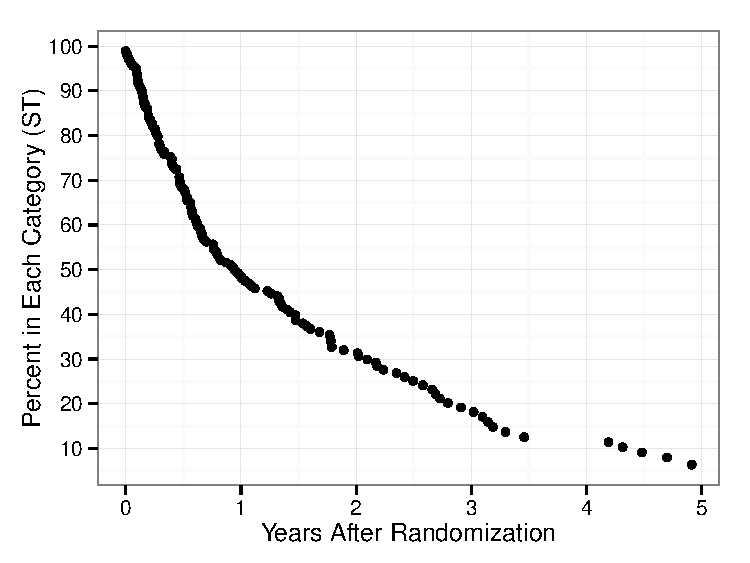
\includegraphics[width=\maxwidth]{figure/beamer-points-1} 

}

\caption[Point Plot]{Point Plot\label{F:points}}
\end{figure}


\end{knitrout}
The \code{aes()} mechanism is a powerful way to communicate data level assignment to \code{geom_} functions. If you want to stratify a dataset by a variable, you can specify that within the \code{aes()} function call using the \code{by=} argument. For points, we often want the stratifying to be either a different \code{color=} or \code{shape=} for stratified data. We can then use the \code{scale_color_} functions (See Section~\ref{S:colors}) or the \code{scale_shape_} functions (See Section~\ref{S:shapes}) to control how these are assigned to the stratifying variable.

Once we have added data to the \code{ggplot} object, we can display the figure as shown in Figure~\ref{F:points}. Until now the figure has been manipulated by sequentially adding function calls to the \code{ccf_plot} object. To display the figure you can either use the \code{show()} function, or simply call the object name at the command line.

Note that we have used the default \emph{shape}, \emph{size} and \emph{color} for this figure. These can be manipulated by adding arguments to the \code{geom_} functions, outside of the \code{aes()} function, as we will demonstrate in the following sections.

\subsection{Error Bars}\label{S:errorbars}

Instead of using a single function to set points, lines and error bars, \pkg{ggplot2} uses individual function calls to control these elements. The \code{geom_errorbar} function takes the same arguments as the other \code{geom_} functions. However, since an errorbar is defined with upper and lower limits, we need to supply an \code{ymax} and \code{ymin} argument to the graphic aesthetic function. This code chunk plots both points, and error bars for the next two data series, the \code{sgdead1} variable with error bars running from \code{stldead1} to \code{studead1} and \code{sgstrk1} variable with error bars running from \code{stlstrk1} to \code{stustrk1}. As we see in Figure~\ref{F:errorBars}, both series were added in \code{color="blue"} (Section~\ref{S:colors}), with different point shapes \code{shape=1} and \code{shape=0} for each series (Section~\ref{S:shapes}). We manipulated the error bar size with the \code{width} argument

\begin{knitrout}\footnotesize
\definecolor{shadecolor}{rgb}{0.969, 0.969, 0.969}\color{fgcolor}\begin{kframe}
\begin{alltt}
\hlcom{#     tuple set=green, symbol=circle, symbsize=1/2, linepe=0, linecl=0,}
\hlcom{#       ebarsize=3/4, ebar=1,}
\hlcom{#       x=iv_state, y=sgdead1, cll=stldead1, clu=studead1, color=blue, end;}
\hlstd{ccf_plot} \hlkwb{<-} \hlstd{ccf_plot} \hlopt{+}
  \hlkwd{geom_point}\hlstd{(}\hlkwc{data}\hlstd{=nonparametric,} \hlkwd{aes}\hlstd{(}\hlkwc{x}\hlstd{=iv_state,} \hlkwc{y}\hlstd{=sgdead1),}\hlkwc{color}\hlstd{=}\hlstr{"blue"}\hlstd{,}\hlkwc{shape}\hlstd{=}\hlnum{1}\hlstd{)} \hlopt{+}
  \hlkwd{geom_errorbar}\hlstd{(}\hlkwc{data}\hlstd{=nonparametric,} \hlkwd{aes}\hlstd{(}\hlkwc{x}\hlstd{=iv_state,} \hlkwc{ymin}\hlstd{=stldead1,} \hlkwc{ymax}\hlstd{=studead1),}
                \hlkwc{color}\hlstd{=}\hlstr{"blue"}\hlstd{,} \hlkwc{width}\hlstd{=}\hlnum{.1}\hlstd{)}

\hlcom{#      tuple set=green, symbol=square, symbsize=1/2, linepe=0, linecl=0,}
\hlcom{#       ebarsize=3/4, ebar=1,}
\hlcom{#       x=iv_state, y=sgstrk1, cll=stlstrk1, clu=stustrk1, color=blue, end;}
\hlstd{ccf_plot} \hlkwb{<-} \hlstd{ccf_plot} \hlopt{+}
  \hlkwd{geom_point}\hlstd{(}\hlkwc{data}\hlstd{=nonparametric,} \hlkwd{aes}\hlstd{(}\hlkwc{x}\hlstd{=iv_state,} \hlkwc{y}\hlstd{=sgstrk1),}\hlkwc{color}\hlstd{=}\hlstr{"blue"}\hlstd{,}\hlkwc{shape}\hlstd{=}\hlnum{0}\hlstd{)} \hlopt{+}
  \hlkwd{geom_errorbar}\hlstd{(}\hlkwc{data}\hlstd{=nonparametric,} \hlkwd{aes}\hlstd{(}\hlkwc{x}\hlstd{=iv_state,} \hlkwc{ymin}\hlstd{=stlstrk1,} \hlkwc{ymax}\hlstd{=stustrk1),}
                \hlkwc{color}\hlstd{=}\hlstr{"blue"}\hlstd{,} \hlkwc{width}\hlstd{=}\hlnum{.1}\hlstd{)}

\hlkwd{show}\hlstd{(ccf_plot)}
\end{alltt}


{\ttfamily\noindent\color{warningcolor}{Warning: Removed 7 rows containing missing values (geom\_point).}}

{\ttfamily\noindent\color{warningcolor}{Warning: Removed 117 rows containing missing values (geom\_point).}}\end{kframe}\begin{figure}[htpb]

{\centering 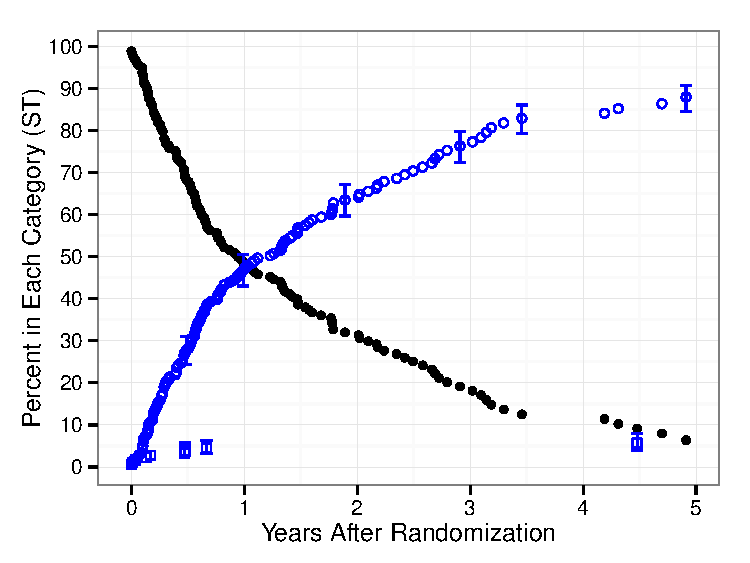
\includegraphics[width=\maxwidth]{figure/beamer-errorBars-1} 

}

\caption[Error Bar Plot]{Error Bar Plot\label{F:errorBars}}
\end{figure}


\end{knitrout}

Note that the \code{x} variable is the same (\code{iv_state}) for all three data series as well as the associated error bars. This is not a requirement, as we could have specified a different variable name for each \code{geom_} function call. Also note that just as in the \code{plot.sas} macro, since we do not want an error bar placed at at every data point, a large number points have the upper and lower error bar y values have been set to missing (\code{NA}). The \pkg{ggplot2} package does print warning messages when we attempt to plot a series with missing values. We typically suppress those warnings, but left them here for illustration purposes only.

\subsection{Lines}\label{S:lines}
Similar to points and error bars, the \code{geom_line} function is used to plot lines. We use the \code{linetype} argument to specify the line styles (Section~\ref{S:linetypes}). We do have to generate a separate \code{geom_line} function call for each limit of the confidence limit, since it is constructed of two lines (the upper and lower confidence limit). The resulting graph is shown in Figure~\ref{F:lines}.
\begin{knitrout}\footnotesize
\definecolor{shadecolor}{rgb}{0.969, 0.969, 0.969}\color{fgcolor}\begin{kframe}
\begin{alltt}
\hlcom{# /**********PARAMETRIC : SOLID LINES AND CONFIDENCE INTERVALS**********/      }
\hlcom{# tuple set=all, x=years, y=noinit, cll=clinit, clu=cuinit,}
\hlcom{# width=0.5,color=black, end;}

\hlstd{ccf_plot} \hlkwb{<-} \hlstd{ccf_plot}\hlopt{+}
  \hlkwd{geom_line}\hlstd{(}\hlkwc{data}\hlstd{=parametric,} \hlkwd{aes}\hlstd{(}\hlkwc{x}\hlstd{=years,} \hlkwc{y}\hlstd{=noinit))}\hlopt{+}
  \hlkwd{geom_line}\hlstd{(}\hlkwc{data}\hlstd{=parametric,} \hlkwd{aes}\hlstd{(}\hlkwc{x}\hlstd{=years,} \hlkwc{y}\hlstd{=clinit),} \hlkwc{linetype}\hlstd{=}\hlstr{"dashed"}\hlstd{)}\hlopt{+}
  \hlkwd{geom_line}\hlstd{(}\hlkwc{data}\hlstd{=parametric,} \hlkwd{aes}\hlstd{(}\hlkwc{x}\hlstd{=years,} \hlkwc{y}\hlstd{=cuinit),} \hlkwc{linetype}\hlstd{=}\hlstr{"dashed"}\hlstd{)}
\hlcom{# }
\hlcom{# tuple set=all, x=years, y=nodeath, cll=cldeath, clu=cudeath,}
\hlcom{# width=0.5,color=blue, end;}
\hlstd{ccf_plot} \hlkwb{<-} \hlstd{ccf_plot}\hlopt{+}
  \hlkwd{geom_line}\hlstd{(}\hlkwc{data}\hlstd{=parametric,} \hlkwd{aes}\hlstd{(}\hlkwc{x}\hlstd{=years,} \hlkwc{y}\hlstd{=nodeath),} \hlkwc{color}\hlstd{=}\hlstr{"blue"}\hlstd{)}\hlopt{+}
  \hlkwd{geom_line}\hlstd{(}\hlkwc{data}\hlstd{=parametric,} \hlkwd{aes}\hlstd{(}\hlkwc{x}\hlstd{=years,} \hlkwc{y}\hlstd{=cldeath),} \hlkwc{linetype}\hlstd{=}\hlstr{"dashed"}\hlstd{,} \hlkwc{color}\hlstd{=}\hlstr{"blue"}\hlstd{)}\hlopt{+}
  \hlkwd{geom_line}\hlstd{(}\hlkwc{data}\hlstd{=parametric,} \hlkwd{aes}\hlstd{(}\hlkwc{x}\hlstd{=years,} \hlkwc{y}\hlstd{=cudeath),} \hlkwc{linetype}\hlstd{=}\hlstr{"dashed"}\hlstd{,} \hlkwc{color}\hlstd{=}\hlstr{"blue"}\hlstd{)}
\hlcom{# }
\hlcom{# tuple set=all, x=years, y=nostrk, cll=clstrk, clu=custrk,}
\hlcom{# linecl=2, width=0.5,color=blue, end;}
\hlstd{ccf_plot} \hlkwb{<-} \hlstd{ccf_plot}\hlopt{+}
  \hlkwd{geom_line}\hlstd{(}\hlkwc{data}\hlstd{=parametric,} \hlkwd{aes}\hlstd{(}\hlkwc{x}\hlstd{=years,} \hlkwc{y}\hlstd{=nostrk),} \hlkwc{color}\hlstd{=}\hlstr{"blue"}\hlstd{)}\hlopt{+}
  \hlkwd{geom_line}\hlstd{(}\hlkwc{data}\hlstd{=parametric,} \hlkwd{aes}\hlstd{(}\hlkwc{x}\hlstd{=years,} \hlkwc{y}\hlstd{=clstrk),} \hlkwc{linetype}\hlstd{=}\hlstr{"dashed"}\hlstd{,} \hlkwc{color}\hlstd{=}\hlstr{"blue"}\hlstd{)}\hlopt{+}
  \hlkwd{geom_line}\hlstd{(}\hlkwc{data}\hlstd{=parametric,} \hlkwd{aes}\hlstd{(}\hlkwc{x}\hlstd{=years,} \hlkwc{y}\hlstd{=custrk),} \hlkwc{linetype}\hlstd{=}\hlstr{"dashed"}\hlstd{,} \hlkwc{color}\hlstd{=}\hlstr{"blue"}\hlstd{)}

\hlkwd{show}\hlstd{(ccf_plot)}
\end{alltt}
\end{kframe}\begin{figure}[htpb]

{\centering 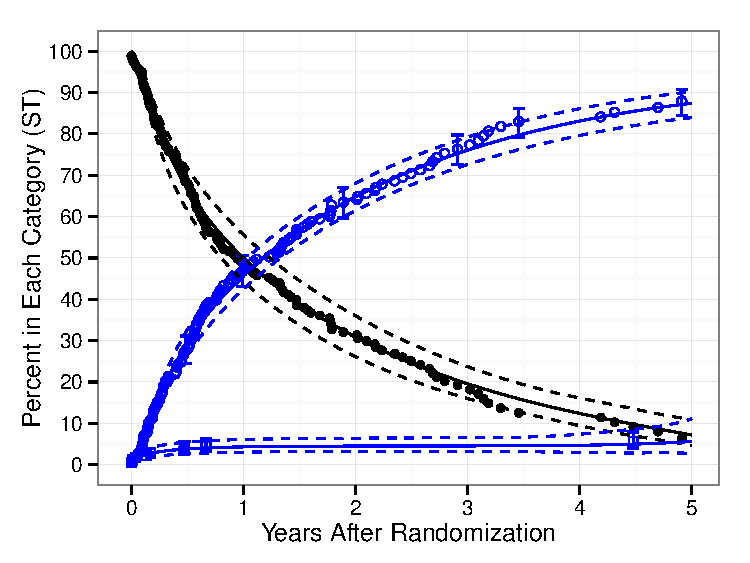
\includegraphics[width=\maxwidth]{figure/beamer-lines-1} 

}

\caption[Line Plot with confidence bands]{Line Plot with confidence bands\label{F:lines}}
\end{figure}


\end{knitrout}

Alternatively, we could use the \code{geom_ribbon} to generate a confidence band using a shaded region with only a single call. The aesthetic argument for \code{geom_ribbon} takes a \code{ymax} and \code{ymin} argument just as the \code{geom_errorbar} function. Note that we used a different data set (\code{data=parametric}) to use a different set of points for generating these lines. 

\subsection{Line types}\label{S:linetypes}
The \code{linetype} argument takes a named string as a value, to set the different line styles. We show a set of frequently used styles in Figure~\ref{F:linetypes} for reference.
\begin{knitrout}\footnotesize
\definecolor{shadecolor}{rgb}{0.969, 0.969, 0.969}\color{fgcolor}\begin{figure}[htpb]

{\centering 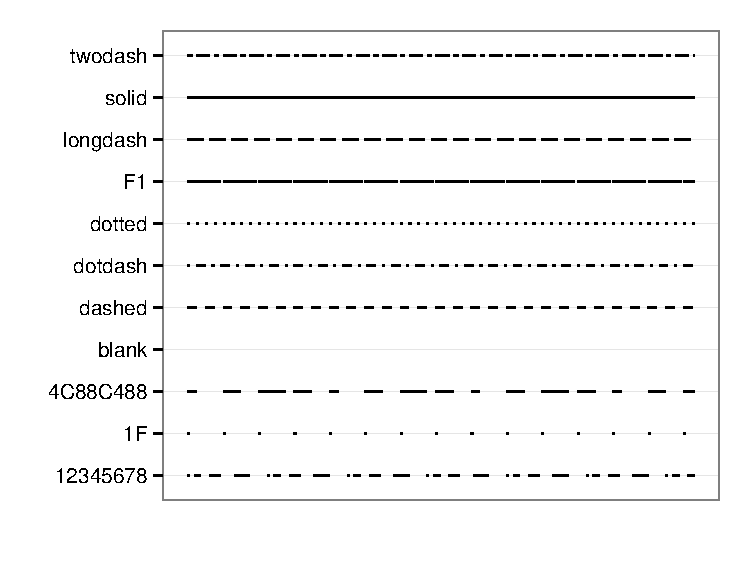
\includegraphics[width=\maxwidth]{figure/beamer-linetypes-1} 

}

\caption[ggplot2 linetype table]{ggplot2 linetype table\label{F:linetypes}}
\end{figure}


\end{knitrout}

\subsection{Shapes}\label{S:shapes}
The \code{shape} argument takes numeric arguments. Though not user friendly, this method is at least consistent. Figure~\ref{F:shapes} shows a catalog of shapes with corresponding numeric argument constructed using the ones place from the x-axis, and tens from the y-axis. For example, the filled dot, default point shape shown in black in Figure~\ref{F:lines} is shape 20.

\begin{knitrout}\footnotesize
\definecolor{shadecolor}{rgb}{0.969, 0.969, 0.969}\color{fgcolor}\begin{figure}[htpb]

{\centering 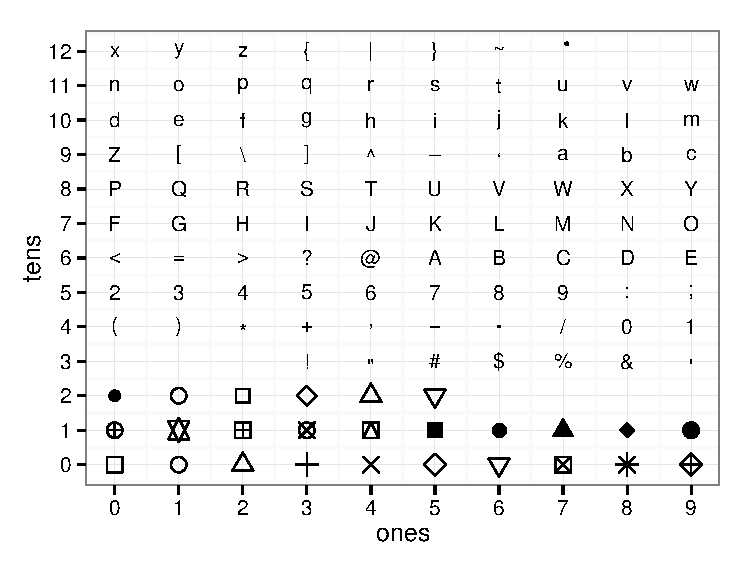
\includegraphics[width=\maxwidth]{figure/beamer-shapes-1} 

}

\caption[ggplot2 shape table]{ggplot2 shape table\label{F:shapes}}
\end{figure}


\end{knitrout}

\subsection{Colors}\label{S:colors}
You can specify colors in \proglang{R} by numeric index, name (as we have done), hexadecimal, or RGB specification. For example \code{col=1} and \code{col="white"}  are equivalent. The chart in Figure~\ref{F:colorChart} was produced with code developed by~\cite{Glynn:2005}. See his \proglang{R}  Color Chart website for all the details you would ever need about using colors in R.

\begin{knitrout}\footnotesize
\definecolor{shadecolor}{rgb}{0.969, 0.969, 0.969}\color{fgcolor}\begin{figure}[htpb]

{\centering 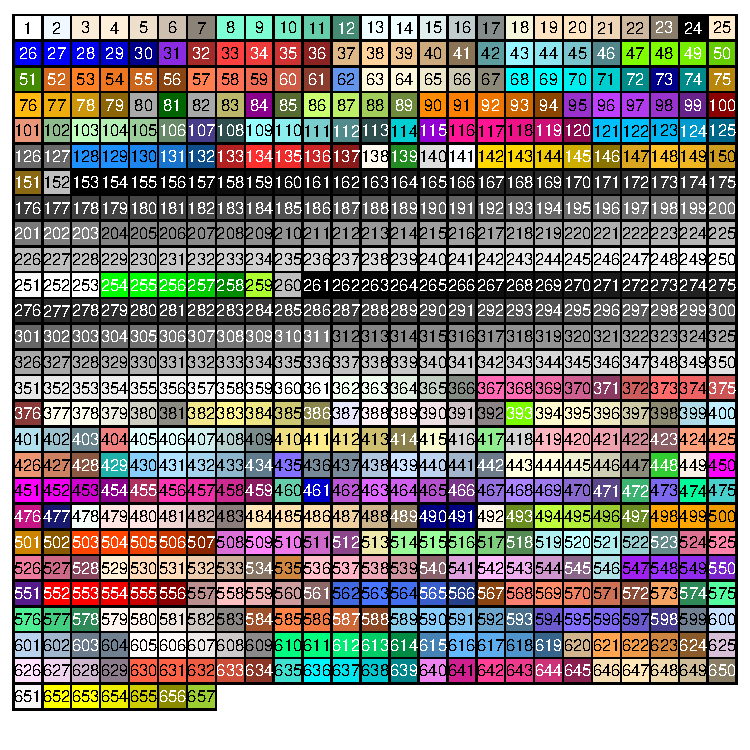
\includegraphics[width=\maxwidth]{figure/beamer-colorChart-1} 

}

\caption[R colors]{R colors\label{F:colorChart}}
\end{figure}


\end{knitrout}

Color theory encompasses a multitude of definitions, concepts and design applications - enough to fill several encyclopedias. However, there are three basic categories of color theory that are logical and useful : The color wheel, color harmony, and the context of how colors are used. ColorBrewer~\citep{Brewer:2003} is an online tool~(\url{http://colorbrewer2.org/}) designed to help people select good color schemes for maps and other graphics. We encourage the use of ColorBrewer as a good, safe introduction to selecting colors based on theoretically good practices. 

The \pkg{RColorBrewer} package~\citep{Neuwirth:2011} simplifies the selection of ColorBrewer colors into \proglang{R}. We have used \pkg{RColorBrewer} to get a list of colors, and assign colors manually to specific variable values using the \pkg{ggplot2} \code{aes()} mechanism. The ColorBrewer palettes have also been built into the \pkg{ggplot2} \code{scale_} functions in the \code{scale_color_brewer} function. We have made extensive use of the \code{palette="Set1"} color palette in figures we have generated. There are also a series of other \code{scale_color_} functions in \pkg{ggplot2} to aid the user in selecting good color schemes for many different settings.

\subsection{Global Figure Commands}\label{S:globals}
By default, the \pkg{ggplot2} package adds space to the figures around the data. We often want to remove this space, or focus in on a smaller window of the figure. This is accomplished with the \code{coord_cartesian} function. By specifying the \code{xlim} and/or \code{ylim} coordinates, we can crop the figure into whatever viewport we are interested in without manipulating the original dataset. Figure~\ref{F:global} sets the origin to (0,0) and clips the x axis at 5.1, and the y axis at 101. We have added the .1 and 1 to each axis for aesthetic reasons to avid chopping off the tick labels when they occur at the end of the viewport.
\begin{knitrout}\footnotesize
\definecolor{shadecolor}{rgb}{0.969, 0.969, 0.969}\color{fgcolor}\begin{kframe}
\begin{alltt}
\hlcom{# Special commands to force origin to 0,0}
\hlstd{ccf_plot} \hlkwb{<-} \hlstd{ccf_plot} \hlopt{+}
  \hlkwd{coord_cartesian}\hlstd{(}\hlkwc{xlim}\hlstd{=}\hlkwd{c}\hlstd{(}\hlnum{0}\hlstd{,}\hlnum{5.1}\hlstd{),} \hlkwc{ylim}\hlstd{=}\hlkwd{c}\hlstd{(}\hlnum{0}\hlstd{,}\hlnum{101}\hlstd{))}

\hlkwd{show}\hlstd{(ccf_plot)}
\end{alltt}
\end{kframe}\begin{figure}[htpb]

{\centering 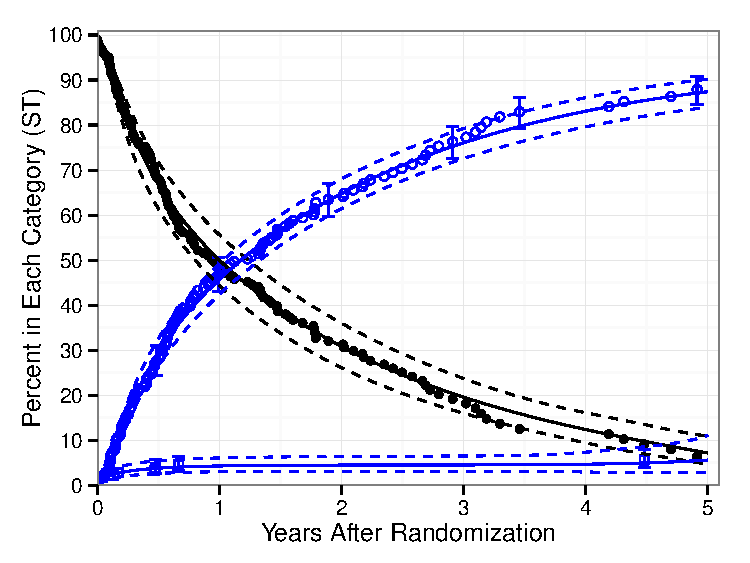
\includegraphics[width=\maxwidth]{figure/beamer-global_-1} 

}

\caption[Adjusting the viewport]{Adjusting the viewport\label{F:global,}}
\end{figure}


\end{knitrout}

% #   expand_limits(x = 0, y = 0) +
% #   scale_x_continuous(expand = c(-0.1, 0.1)) + 
% #   scale_y_continuous(expand = c(-1, 0.1))

\subsection{PowerPoint Figures}\label{S:powerPointFigures}

As a second example, we recreate a figure that was created for PowerPoint with the \code{plot.sas} macro. In most cases, we do not include points when generating presentation figures, so this figure was generated with only \code{geom_line} function calls. We also show how the figure can be created in a single set of function calls.

\begin{knitrout}\footnotesize
\definecolor{shadecolor}{rgb}{0.969, 0.969, 0.969}\color{fgcolor}\begin{kframe}
\begin{alltt}
\hlcom{# %plot(goptions gsfmode=replace, device=cgmmppa, ftext=hwcgm001, end;}
\hlcom{# axisx order=(0 to 5 by 1), minor=none, value=(height=2.4), end;}
\hlcom{# axisy order=(0 to 100 by 20), minor=none, value=(height=2.4), }
\hlcom{# value=(height=2.4 j=r ' ' '20' '40' '60' '80' '100'), end;}
\hlcom{# tuple set=all, x=years, y=noinit, width=3, color=gray, end;}
\hlcom{# tuple set=all, x=years, y=nostrk, width=3, color=red, end;}
\hlcom{# tuple set=all, x=years, y=nodeath, width=3, color=blue, end;}
\hlcom{# );}
\hlstd{ccf_pptPlot} \hlkwb{<-} \hlkwd{ggplot}\hlstd{()}\hlopt{+}
  \hlkwd{scale_x_continuous}\hlstd{(}\hlkwc{breaks}\hlstd{=}\hlkwd{seq}\hlstd{(}\hlnum{0}\hlstd{,}\hlnum{5}\hlstd{,}\hlnum{1}\hlstd{))}\hlopt{+}
  \hlkwd{scale_y_continuous}\hlstd{(}\hlkwc{breaks}\hlstd{=}\hlkwd{seq}\hlstd{(}\hlnum{0}\hlstd{,}\hlnum{100}\hlstd{,}\hlnum{20}\hlstd{))}\hlopt{+}
  \hlkwd{geom_line}\hlstd{(}\hlkwc{data}\hlstd{=parametric,} \hlkwd{aes}\hlstd{(}\hlkwc{x}\hlstd{=years,} \hlkwc{y}\hlstd{=noinit),} \hlkwc{color}\hlstd{=}\hlstr{"grey"}\hlstd{,} \hlkwc{size}\hlstd{=}\hlnum{1.5}\hlstd{)}\hlopt{+}
  \hlkwd{geom_line}\hlstd{(}\hlkwc{data}\hlstd{=parametric,} \hlkwd{aes}\hlstd{(}\hlkwc{x}\hlstd{=years,} \hlkwc{y}\hlstd{=nostrk),} \hlkwc{color}\hlstd{=}\hlstr{"red"}\hlstd{,} \hlkwc{size}\hlstd{=}\hlnum{1.5}\hlstd{)}\hlopt{+}
  \hlkwd{geom_line}\hlstd{(}\hlkwc{data}\hlstd{=parametric,} \hlkwd{aes}\hlstd{(}\hlkwc{x}\hlstd{=years,} \hlkwc{y}\hlstd{=nodeath),} \hlkwc{color}\hlstd{=}\hlstr{"blue"}\hlstd{,} \hlkwc{size}\hlstd{=}\hlnum{1.5}\hlstd{)}

\hlkwd{show}\hlstd{(ccf_pptPlot)}
\end{alltt}
\end{kframe}\begin{figure}[htpb]

{\centering 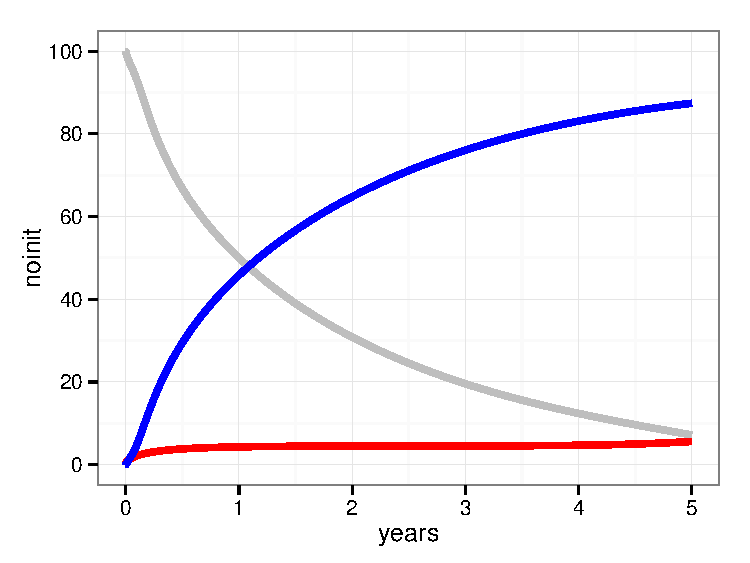
\includegraphics[width=\maxwidth]{figure/beamer-powerpoint-1} 

}

\caption[PowerPoint Figures]{PowerPoint Figures\label{F:powerpoint}}
\end{figure}


\end{knitrout}


% -----------------------------------------------------
\section[Themes for publications]{\pkg{ggplot2} themes for publication}\label{S:themes}
% -----------------------------------------------------
The themes system in \pkg{ggplot2} enables a user to control non-data elements of a \code{ggplot} object. Where we use color palettes (Section~\ref{S:colors}), shapes (Section~\ref{S:shapes}) and linetypes (Section~\ref{S:linetypes}) to control the data elements, we use themes to control the visual details of most of the remaining aspects of our figures. 

The \pkg{hviPlotR} package contains two custom themes. The \code{theme_man()} theme is used for manuscripts, and the \code{theme_ppt()} theme is used for powerpoint documents. These themes can be applied to any figure that was created using the \pkg{ggplot2} package.  

\subsection{Theme for Manuscripts}\label{S:theme_man}

As before, there are multiple ways to assign a theme to use. Using the \code{theme_set()} function will apply the theme for all subsequent figures. Even if the figure was created before the \code{theme_set} call, displaying a figure after the call will apply the new theme. It is then best to revert to the default theme when at the end of a section. The following code chunk demonstrates this process using the manuscript theme (\code{theme_man()}). The resulting manuscript graphic is show in Figure~\ref{F:manuscriptTheme}.
\begin{knitrout}\footnotesize
\definecolor{shadecolor}{rgb}{0.969, 0.969, 0.969}\color{fgcolor}\begin{kframe}
\begin{alltt}
\hlcom{# Set the theme for manuscripts,}
\hlkwd{theme_set}\hlstd{(}\hlkwd{theme_man}\hlstd{())}

\hlcom{# show the figure.}
\hlstd{ccf_plot}

\hlcom{# Reset the theme to the resonable default used previously.}
\hlkwd{theme_set}\hlstd{(}\hlkwd{theme_bw}\hlstd{())}
\end{alltt}
\end{kframe}\begin{figure}[htpb]

{\centering 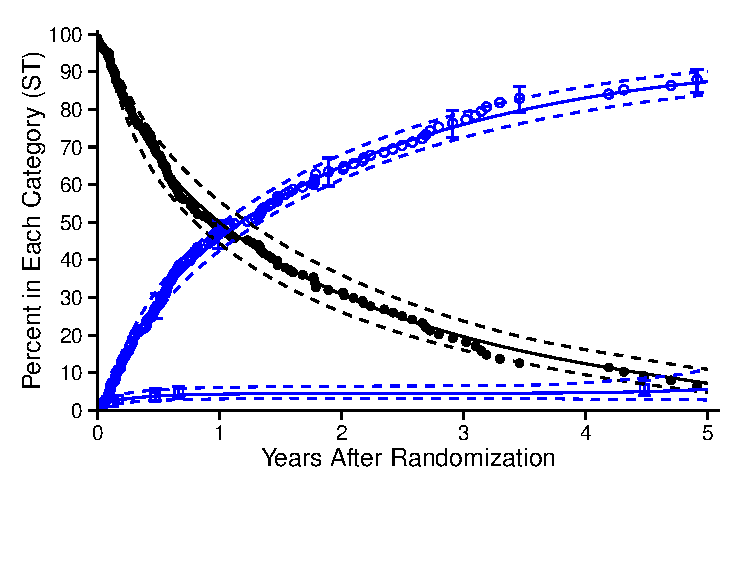
\includegraphics[width=\maxwidth]{figure/beamer-manuscriptTheme-1} 

}

\caption[Theme for Manuscripts]{Theme for Manuscripts\label{F:manuscriptTheme}}
\end{figure}


\end{knitrout}

Note that we are plotting the same figure show in Figure~\ref{F:global}. However, we have modified the box around the plot window as well as made some other minor modifications targeted at creating publication quality graphics. 

\subsection{Theme for Presentations}\label{S:theme_ppt}

In this example, we apply the powerpoint theme to only effect the figure constructed in Figure~\ref{F:powerpoint}. This code chunk removes the x and y axis label, since we prefer to add those within PowerPoint directly. The results are shown in Figure~\ref{F:powerpointThemeC}.
\begin{knitrout}\footnotesize
\definecolor{shadecolor}{rgb}{0.969, 0.969, 0.969}\color{fgcolor}\begin{kframe}
\begin{alltt}
\hlcom{# Update the PowerPoint Figure to include the PPT Theme, and remove axis labels.}
\hlcom{# Axis labels will be added manually in powerpoint.}
\hlstd{ccf_pptPlot} \hlkwb{<-} \hlstd{ccf_pptPlot}\hlopt{+}
  \hlkwd{labs}\hlstd{(}\hlkwc{x}\hlstd{=}\hlstr{""}\hlstd{,}\hlkwc{y}\hlstd{=}\hlstr{""}\hlstd{)}\hlopt{+}
  \hlkwd{theme_ppt}\hlstd{()}

\hlstd{ccf_pptPlot}
\end{alltt}
\end{kframe}\begin{figure}[htpb]

{\centering 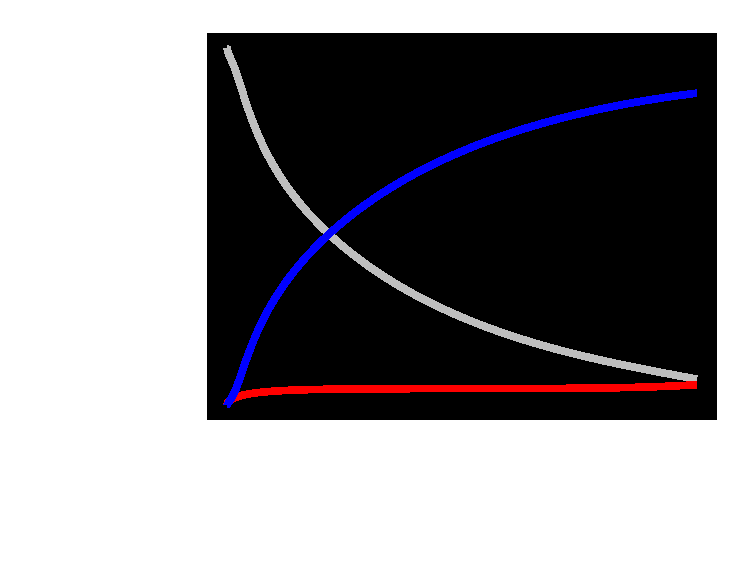
\includegraphics[width=\maxwidth]{figure/beamer-powerpointThemeC-1} 

}

\caption[PowerPoint theme]{PowerPoint theme\label{F:powerpointThemeC}}
\end{figure}


\end{knitrout}


The theme for presentations is significantly different from what we showed in Figure~\ref{F:powerpoint}. Since our presentations are displayed on a blue background, we have changed the axis tick labels to white. The axis labels, frame and tick mark are there, on an invisible background so that changes to the slide background are visible through the figure.  To see the full effect, we modify the theme of the plot background from "transparent" to "blue" in Figure~\ref{F:powerpointThemeC}.
\begin{knitrout}\footnotesize
\definecolor{shadecolor}{rgb}{0.969, 0.969, 0.969}\color{fgcolor}\begin{kframe}
\begin{alltt}
\hlcom{# Show the figure... the theme statement is used so the axis tick marks and values}
\hlcom{# are visible in this document.}
\hlstd{ccf_pptPlot} \hlopt{+}
  \hlkwd{theme}\hlstd{(}\hlkwc{plot.background} \hlstd{=} \hlkwd{element_rect}\hlstd{(}\hlkwc{fill}\hlstd{=}\hlstr{'blue'}\hlstd{,} \hlkwc{colour}\hlstd{=}\hlstr{'blue'}\hlstd{))}
\end{alltt}
\end{kframe}\begin{figure}[htpb]

{\centering 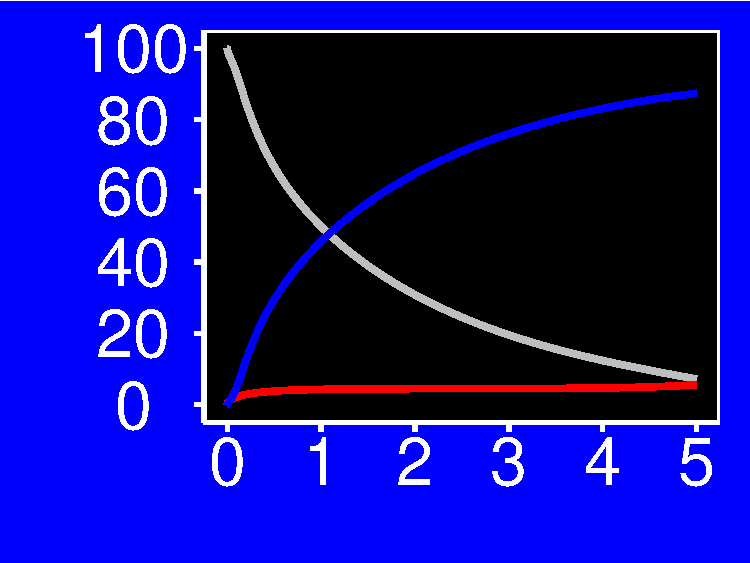
\includegraphics[width=\maxwidth]{figure/beamer-powerpointTheme-1} 

}

\caption[Theme for Presentations]{Theme for Presentations\label{F:powerpointTheme}}
\end{figure}


\end{knitrout}

% -----------------------------------------------------
\section{Saving Publication graphics}\label{S:saving}
% -----------------------------------------------------

Once we have created the figure, and formatted it as desired (using a \pkg{hviPlotR} theme), we need to save the figure in a format that can easily be imported into our publications. 

\subsection{Manuscript graphics}

It is a best practice that we include a footnote containing the figure path in each figure we save. This way, when a user sends the file to a collaborator, we can reverse engineer where the file and generating code resides in case changes are required. We use the \pkg{gridExtra} package~\citep{Auguie:2012} to add this footnote with the following recipe.
\begin{knitrout}\footnotesize
\definecolor{shadecolor}{rgb}{0.969, 0.969, 0.969}\color{fgcolor}\begin{kframe}
\begin{alltt}
\hlkwd{library}\hlstd{(gridExtra)}

\hlstd{ccf_savePlot} \hlkwb{<-} \hlkwd{arrangeGrob}\hlstd{(ccf_plot}\hlopt{+}\hlkwd{theme_man}\hlstd{(),}
                            \hlkwc{sub} \hlstd{=} \hlkwd{textGrob}\hlstd{(}\hlkwd{paste}\hlstd{(}\hlkwd{getwd}\hlstd{(),} \hlkwd{Sys.Date}\hlstd{(),} \hlkwc{sep}\hlstd{=}\hlstr{" "}\hlstd{),}
                                           \hlkwc{x} \hlstd{=} \hlnum{0}\hlstd{,} \hlkwc{hjust} \hlstd{=} \hlopt{-}\hlnum{.1}\hlstd{,} \hlkwc{vjust}\hlstd{=}\hlnum{.01}\hlstd{,}
                                           \hlkwc{gp} \hlstd{=} \hlkwd{gpar}\hlstd{(}\hlkwc{fontface} \hlstd{=} \hlstr{"italic"}\hlstd{,} \hlkwc{fontsize} \hlstd{=} \hlnum{6}\hlstd{)))}
\hlstd{ccf_savePlot}
\end{alltt}
\end{kframe}\begin{figure}[htpb]

{\centering 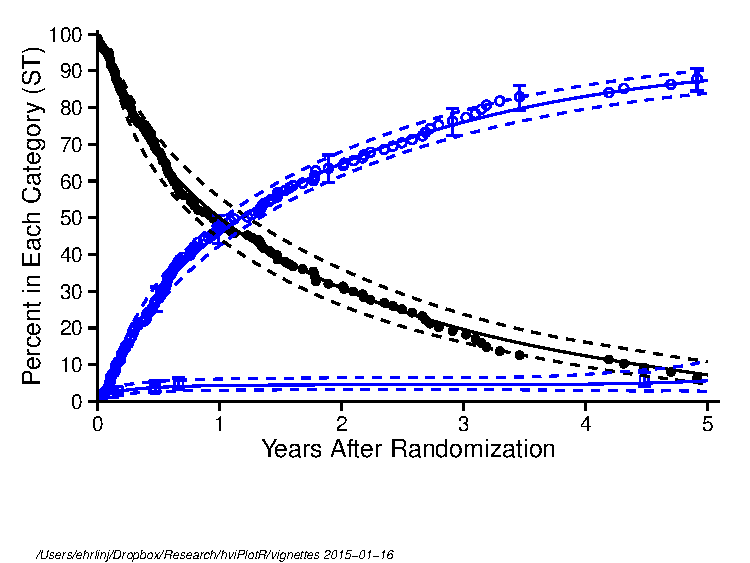
\includegraphics[width=\maxwidth]{figure/beamer-manuscriptFootnote-1} 

}

\caption[Manuscript figure format with path footnote]{Manuscript figure format with path footnote.\label{F:manuscriptFootnote}}
\end{figure}


\end{knitrout}
Figure~\ref{F:manuscriptFootnote} uses the same plot in Figure~\ref{F:manuscriptTheme} with the code \code{ccf_plot+theme_man()}. The current working directory is obtained using the \code{getwd()} function. The \code{Sys.Date()} function returns the system date for timestamping the figure. The footnote is placed with the \code{x = 0, hjust = -.1, vjust=.01,} and formatted with the \code{gp = gpar(fontface = "italic", fontsize = 6)}.

For Word documents (Office $\ge 2007$) we can import PDF graphics as a vector based format. Saving the figure is accomplished using either the \code{ggsave} function, or the \code{pdf(); show();dev.off()} combination. We have a specific set of \code{width} and \code{height} dimensions required for saving the figure with footnote included to get the font sizes to import correctly in Word. 
\begin{knitrout}\footnotesize
\definecolor{shadecolor}{rgb}{0.969, 0.969, 0.969}\color{fgcolor}\begin{kframe}
\begin{alltt}
\hlkwd{ggsave}\hlstd{(}\hlkwc{filename}\hlstd{=}\hlstr{"manuscript.pdf"}\hlstd{,}
       \hlkwc{height}\hlstd{=}\hlnum{4}\hlstd{,} \hlkwc{width}\hlstd{=}\hlnum{5}\hlstd{,}
       \hlstd{ccf_savePlot)}
\end{alltt}
\end{kframe}
\end{knitrout}


\subsection{PowerPoint graphics}
We use the \pkg{ReporteRs} package~\citep{Gohel:2014} to insert vector based figures from \proglang{R} into PowerPoint documents. The latest version of the \pkg{ReporteRs} package is available from \url{http://davidgohel.github.io/ReporteRs/}. We install this package as we installed the \pkg{hviPlotR} package.
\begin{knitrout}\footnotesize
\definecolor{shadecolor}{rgb}{0.969, 0.969, 0.969}\color{fgcolor}\begin{kframe}
\begin{alltt}
\hlcom{# Install the latest ReporteRs package.}
\hlcom{#}
\hlcom{# The devtools package is installed on all our }
\hlcom{# jjnb-gen servers as well as other R instances.}
\hlkwd{library}\hlstd{(devtools)}

\hlcom{# To get the latest version.}
\hlkwd{install_github}\hlstd{(}\hlstr{"davidgohel/ReporteRs"}\hlstd{)}
\end{alltt}
\end{kframe}
\end{knitrout}

Basically, the package works by opening a saved PowerPoint Presentation, and inserting new slides containing graphs or tables into the document. The resulting document is then saved to a new presentation. We then pass this presentation to our collaborators, who then copy and paste the \pkg{ggplot2} slides into their own presentations. 

The \pkg{ggplot2} graphics that are inserted into the presentation are converted into an editable vector based format. When the document is edited in PowerPoint, graphical components like points, lines, text can be easily modified to match the presenters style.

The following code block is an \proglang{R} recipe for saving the \code{ccf_pptPlot} created in Section~\ref{S:theme_ppt}. 
\begin{knitrout}\footnotesize
\definecolor{shadecolor}{rgb}{0.969, 0.969, 0.969}\color{fgcolor}\begin{kframe}
\begin{alltt}
\hlkwd{library}\hlstd{(ReporteRs)}
\hlcom{# Create a powerPoint document using ../inst/RDPresentation.pptx }
\hlcom{# as a template document.}
\hlstd{doc} \hlkwb{=} \hlkwd{pptx}\hlstd{(}\hlkwc{template}\hlstd{=}\hlkwd{paste}\hlstd{(}\hlstr{"../inst/RDPresentation.pptx"}\hlstd{,} \hlkwc{sep}\hlstd{=}\hlstr{""}\hlstd{))}

\hlcom{# Here we define powerpoint document filename to write}
\hlcom{# the presentation. This will be overwritten}
\hlstd{pptx.file} \hlkwb{=} \hlkwd{paste}\hlstd{(}\hlstr{"RDExample.pptx"}\hlstd{,} \hlkwc{sep}\hlstd{=}\hlstr{""}\hlstd{)}

\hlcom{##--------}
\hlcom{# For each graph, addSlide. The graphs require the }
\hlcom{# “Title and Content” template.}
\hlstd{doc} \hlkwb{=} \hlkwd{addSlide}\hlstd{( doc,} \hlstr{"Title and Content"} \hlstd{)}

\hlcom{# Place a title}
\hlstd{doc} \hlkwb{=} \hlkwd{addTitle}\hlstd{( doc,} \hlstr{"Treatment Difference"} \hlstd{)}

\hlcom{# Now add the graph into the powerPoint doc }
\hlstd{doc} \hlkwb{=} \hlkwd{addPlot}\hlstd{(} \hlkwc{doc}\hlstd{=doc,} \hlkwc{fun}\hlstd{=print,}
               \hlkwc{x}\hlstd{=ccf_pptPlot}\hlopt{+}\hlkwd{theme_ppt}\hlstd{() ,}
               \hlkwc{editable} \hlstd{=} \hlnum{TRUE}\hlstd{,}
               \hlkwc{offx}\hlstd{=}\hlnum{.75}\hlstd{,} \hlkwc{offy}\hlstd{=}\hlnum{1.1}\hlstd{,} \hlkwc{width}\hlstd{=}\hlnum{8}\hlstd{,} \hlkwc{height}\hlstd{=}\hlnum{6}\hlstd{)}
\hlcom{##--------}
\hlcom{## IF you want to add more, just repeat between the ##-------- comments}
\hlcom{##--------}

\hlcom{# write the output powerpoint doc. }
\hlcom{# This will not overwrite an open document, since open PPT files are locked.}
\hlkwd{writeDoc}\hlstd{( doc, pptx.file )}
\end{alltt}
\end{kframe}
\end{knitrout}

The only modification possibly require for this recipe may be moving the insertion point (\code{offx} and \code{offy} arguments) and/or size (\code{width} and \code{height}) of the figure in the \code{addPlot()} function call.
% 
% % -----------------------------------------------------
% \section{Generating other figure types}\label{S:alternateFigures}
% % -----------------------------------------------------
% 
% \subsection{Bar Charts}
% \code{geom_boxplot} \code{geom_bar}
% 
% \subsection{Histograms}
% \code{geom_histogram}
% 
% \subsection{Additional Figure Types}
% 

% -----------------------------------------------------
\section{Graphics rules to live by}\label{S:rules}
% -----------------------------------------------------
This section is in progress\ldots

% =======================================
\section{Conclusions} \label{S:concl}
% =======================================

In this article, we present the \pkg{hviPlotR} package for \proglang{R}. The package is made up of \pkg{ggplot2} themes for publication quality graphics, as well as this tutorial document included as a package vignette. The package is available from \url{https://github.com/ehrlinger/hviPlotR} and can be installed using the \code{devtools::install_github("ehrlinger/hviPlotR")} command. 

% =======================================
% \section{Literatur} \label{sec: references}
% =======================================
%\nocite{*}

\bibliography{hviPlotR}



\end{document}
